%%%%%%%%%%%%%%%%%%%%%%%%%%%%%%%%%%%%%%%%%%%%%%%%%%%%%%%%%%%%%%%%%%%%%%%%%%%%%%%%%%%%%%%%%%%%%%%%%%%
%%%%%%%%%%%%%%%%%%%%%%%%%%%%%%%%%%%%%%%%%%%%%%%%%%%%%%%%%%%%%%%%%%%%%%%%%%%%%%%%%%%%%%%%%%%%%%%%%%%
%%%%%%%%%%%%%%%%%%%%%%%%%%%%%%%%%%%%%%%%%%%%%%%%%%%%%%%%%%%%%%%%%%%%%%%%%%%%%%%%%%%%%%%%%%%%%%%%%%%
%%%%%%%%%%%%%%%%%%%%%%%%%%%%%%%%%%%%%%%%%%%%%%%%%%%%%%%%%%%%%%%%%%%%%%%%%%%%%%%%%%%%%%%%%%%%%%%%%%%

\subsection{Matemáticas}

\begin{proposicion}
Sean $u$ y $v$ dos funciones tipo \textit{pseudo $\delta$ de Dirac}, es decir, unimodales con un
máximo  y (...). Si $u$ tiene una concentración muy alta, con relación a $v$, entonces
\begin{equation*}
\intR u(x) v(x+k) dx \approx v(k) \intR u(x) dx
\end{equation*}
\label{pseudo_d}
\end{proposicion}

\subsubsection{Espectro evolutivo}


\subsubsection{Estimación del espectro evolutivo}

Una vez definido el espectro evolutivo para procesos no-estacionarios con varianza finita,
cabe preguntarse sobre le estimación de esta cantidad a partir de una realización del proceso
usando, por ejemplo, periodogramas modificados;
tal pregunta no tiene, en general, una respuesta satisfactoria.
Es por ello que se
define una colección, más restringida, de procesos no-estacionarios cuyo espectro evolutivo pueda
ser estimado efectivamente usando la técnica de ventanas.

Considerando un proceso no-estacionario \xt que admite una representación de la forma
$X(t) = \intR A(t,\omega) e^{i \omega t} dZ(\omega)$, entonces el espectro evolutivo queda
definido como
\begin{equation}
dF_t(\omega) = \abso{A(t,\omega)}^{2} d\mu(\omega)
\label{esp_evolutivo}
\end{equation}

Antes de poder usar la proposición \ref{pseudo_d} para estimar $F_t$ (con respecto a $t$) usando 
una ventana espectral, hay que medir la dispersión de $F_t$ en el tiempo; más aún, hay que
pedir que esa dispersión sea finita.
Con vista a la ecuación \ref{esp_evolutivo}, se puede usar la conexión entre $F$ y $A$ para
establecer condiciones respecto a la segunda; se define entonces a $H_\omega$, la transformada de
Fourier de $A$ en el tiempo
\begin{equation}
A(t,\omega) = \intR e^{i t \theta} dH_\omega(\theta)
\end{equation}

Un motivo muy fuerte para definir un objeto tan rebuscado es que (...)
%es una función de distribución
%de energía \textit{en las frecuencias}
%
%Vagamente, $H_\omega$ es la transformada de Fourier, en el tiempo, para la transformada de Fourier
%del espectro, en las frecuencias.

Posteriormente se define a $B_{\mathbf{F}}$, el ancho de banda para $H_\omega$ con respecto a la 
familia de funciones $\mathbf{F}$, como

\begin{equation}
B_{\mathbf{F}}(\omega) = \intR \abso{\theta} \abso{dH_\omega(\theta)}
\end{equation}

Se dice que el proceso es semi-estacionario con respecto a $\mathbf{F}$ si 
$\sup_\omega B_{\mathbf{F}} < \infty$. El proceso se dice simplemente \textbf{semi-estacionario} 
si esta cantidad es acotada para cualquier familia de funciones admisibles 
$\mathbf{F} \in \mathbf{C}$; entonces se puede definir la constante $B_X$,
el \textit{ancho de banda característico de} \xt, como

\begin{equation}
B_X = \sup_{\mathbf{F}\in \mathbf{C}} \left[ \sup_\omega B_{\mathbf{F}}(\omega) \right]^{-1}
\end{equation}

Muy vagamente, $B_X$ indica el tiempo máximo en el cual el proceso, representado en la forma
\ref{esp_evolutivo}, (...)

Una vez definida la cantidad $B_X$, y habiendo supuesto que no es 0, es demostrado en
\cite{Priestley65} que el estimador $U$ definido como en ...
satisface que
\begin{equation}
\E{\abso{U(t,\omega)}^{2}} = \intR \abso{\Gamma(\omega)}^{2} f(t,\omega+\omega_0) d\omega
+ \orden\left( \nicefrac{B_g}{B_X} \right)
\end{equation}

De esta última expresión es evidente que el estimador es mejor conforme 
\begin{itemize}
\item  $B_X$, el tiempo
máximo para el cual el proceso es \textit{básicamente estacionario}, es mayor
\item $B_g$, la dispersión en el tiempo para la ventana $g$, es menor
\end{itemize}

---

Entonces se ha probado en \cite{Priestley66,Priestley69} que bajo ciertas
condiciones p

\subsubsection{Prueba de Priestley-Subba Rao}

Una propiedad interesante de poder estimar el espectro evolutivo de un proceso, a partir de
una realización del mismo, es la 
capacidad para identificar si éste pudiera reducirse al
espectro usual, definido para procesos débilmente estacionarios --bastaría
con revisar si el espectro estimado es constante en el tiempo.
%En otras palabras,
%el espectro evolutivo puede usarse como 
%herramienta para decidir si un proceso es estacionario.

La prueba de estacionariedad propuesta por Priestley y Subba Rao en 1969 \cite{Priestley69}
tiene como \textit{ingrediente principal} un estimador muy particular para una cantidad que depende 
del espectro, con
%cambia de forma predecible cuando el proceso es débilmente estacionario y tiene 
propiedades estadísticas adecuadas para detectar la posible estacionariedad.

%Esta prueba fue presentada en 1969 por Priestley y Subba Rao \cite{Priestley69}, y se basa

Sea \xt que se tiene un proceso semi-estacionario y sea \xtd un conjunto de observaciones
del proceso, espaciadas uniformemente en el tiempo.
% de manera uniforme con $t_{i+1}-t_i = \Delta_t$.
Se construye a $\widehat{f}$, el estimador de doble ventana definido como en la sección anterior,
usando las funciones ventana $g_h$ y $w_\tau$, y sus respectivas transformadas de Fourier
$\Gamma_h$ y $W_\tau$. Como se mencionó previamente, bajo las condiciones descritas se cumple
que $\widehat{f}$ es un estimador consistente y aproximadamente insesgado para $f$, el espectro
evolutivo de \xt. Ahora bien, considerando las siguientes aproximaciones
%
\begin{itemize}
\item $\E{\widehat{f}(t,\omega)} \approx f(t,\omega)$
\item $\Var{\widehat{f}(t,\omega)} \approx 
\frac{C}{T} f^{2}(t,\omega) \intR \abso{\Gamma^{4}(\theta)} d\theta$
\end{itemize}
%
donde $C = \lim_{T\rightarrow \infty} T \intR \abso{W_T(\lambda)} d\lambda$.
Usando a $\widehat{f}$,
se define el estimador $Y$ como el logaritmo de éste, 
$Y(t,\omega) = \log\left(\widehat{f}(t,\omega)\right)$,
y que tiene las siguientes propiedades
%
\begin{itemize}
\item $\E{Y(t,\omega)} \approx \log\left(f(t,\omega)\right)$
\item $\Var{Y(t,\omega)} \approx 
\frac{C}{T} \intR \abso{\Gamma_h(\theta)}^{4} d\theta =: \sigma^{2}$
\end{itemize}
%

Cabe destacar que la varianza $Y$ no es formalmente independiente de $f$, sino que es
\textit{aproximadamente independiente}; en otras palabras, la varianza de $Y$ depende 
\textit{más} del propio estimador que del verdadero valor de $\log\circ f$.
Esto no es tan sorprendente tomando en cuenta el diseño del estimador de doble ventana, que
otorga mayor importancia a la información local usando repetidamente la proposición
\ref{pseudo_d}. Esta independencia asintótica sugiere que $Y$ puede verse como
%
%\begin{equation}
$Y(t,\omega) = \log\left(f(t,\omega) \right) + \varepsilon(t,\omega)$,
%\end{equation}
%
con $\E{\varepsilon(t,\omega)} \approx 0$ y $\Var{\varepsilon(t,\omega)} \approx
\sigma^{2}$.

%Continuando con el estimador $Y$, 
Más aún,
es demostrado en \cite{Priestley66} que si
$\abso{\omega-\omega_0}$ es suficientemente grande como para que
$\intR \abso{\Gamma_h(\theta+\omega)}^{2}\abso{\Gamma_h(\theta+\omega_0)}^{2} d\theta \approx 0$,
entonces 
%
%\begin{itemize}
%\item 
$\Cov{Y(t,\omega),Y(t,\omega_0)} \approx 0$.
%\end{itemize}
%
Similarmente, si $\abso{t-t_0} >> \intR \abso{t} \abso{w_\tau (t)} dt $, entonces
%
%\begin{itemize}
%\item 
$\Cov{Y(t,\omega),Y(t_0,\omega)} \approx 0$.
%\end{itemize}

Bajo estas nuevas condiciones, es posible construir una versión discretizada de $Y$ tal 
que los componentes $\varepsilon$ sean estadísticamente independientes. Para ello se define
una malla de puntos $(t_i,\omega_j)$, con $i = 1,\dots,I$ y  $j=1,\dots,J$, y posteriormente
a la matriz $Y$ como $Y_{i,j} = Y(t_i,\omega_j)$, que satisface
%
\begin{itemize}
\item $Y_{i,j} = \log\left(f(t_i,\omega_j)\right) + \varepsilon_{i,j}$
\item $\E{\varepsilon_{i,j}} \approx 0$
\item $\Var{\varepsilon_{i,j}} \approx \sigma^{2} = 
\frac{C}{T} \intR \abso{\Gamma_h(\theta)}^{4} d\theta$
\item $\Cov{\varepsilon_{i,j},\varepsilon_{i_0,j_0}} \approx 0$ siempre que $(i,j)\neq (i_0,j_0)$
\end{itemize}

Ha sido sugerido por Jenkins [??] que si el número de puntos es suficientemente grande, entonces
las componentes de $Y$ siguen distribuciones aproximadamente normales, de modo que
$\varepsilon_{i,j} \sim N(0,\sigma^{2})$.

Habiendo definido al estimador $Y$ en su versión discretizada, 
%es relativamente fácil
%explicar el funcionamiento de la prueba: si el proceso en cuestión es débilmente estacionario,
%entonces 
es posible definir criterios para idetificar la estacionariedad débil; primero se define 
como hipótesis nula
un modelo
general (puede o no ser estacionario)
%
\begin{equation*}
H_0 : \hspace{1em} Y_{i,j} = \mu + \alpha_i + \beta_j + \gamma_{i,j} + \varepsilon_{i,j}
\end{equation*}
%
donde $\varepsilon$ son como se definieron anteriormente,
$\mu$ el promedio de $Y$ sobre todos tiempos y frecuencias, $\alpha$ y $\beta$ son las 
\textit{variaciones} en el tiempo y las frecuencias, respectivamente, y $\gamma$ representa las
variaciones no-lineales en el tiempo y las frecuencias.
%
%Naturalmente, el primer paso para identificar la estacionariedad es contrastar $H_0$ contra un 
%modelo donde $\gamma$ es negligible, es decir
%%
%\begin{equation*}
%H_1 : \hspace{1em} Y_{i,j} = \mu + \alpha_i + \beta_j + \varepsilon_{i,j}
%\end{equation*}
%%
Si se le otorga a $\varepsilon$ el papel de \textit{absorber los errores} del modelo, el suponer
que alguna u otra componente del modelo general desemboca en uno de varios modelos.

\begin{center}
\begin{tabular}{lcc}
Modelo & Unif. modulado & Estacionario \\
$H_1 : \hspace{1em} Y_{i,j} = \mu + \alpha_i + \beta_j + \varepsilon_{i,j}$ & no & si \\
$H_2 : \hspace{1em} Y_{i,j} = \mu + \alpha_i + \varepsilon_{i,j}$ & si & si \\
$H_3 : \hspace{1em} Y_{i,j} = \mu + \beta_j + \varepsilon_{i,j}$ & no & si \\
\end{tabular}
\end{center}

En procesos uniformemente modulados $Y$ depende linealmente tanto del tiempo como de las
frecuencias, de modo que $f$ depende \textit{multiplicativamente} de estos mismos parámetros;
si bien estos procesos son no-estacionarios, varias procedimientos y estimadores diseñados para 
procesos débilmente estacionarios pueden funcionar sobre ellos, como son los análisis de 
coherencia.

Con respecto a la contrastación de estos modelos, se basa en comparar los valores de $Y$ contra
los diferentes promedios, según el modelo a contrastar.

\begin{center}
\begin{tabular}{lll}
$S_T$ & $= J \sum_{i=1}^{I} \left( Y_{i,\bullet} - Y_{\bullet,\bullet} \right)^{2}$ 
& $\sim \sigma^{2} \chi^{2}(I-1)$ \\
$S_F$ & $= I \sum_{j=1}^{J} \left( Y_{\bullet,j} - Y_{\bullet,\bullet} \right)^{2}$ 
& $\sim \sigma^{2} \chi^{2}(J-1)$ \\
$S_{I+R}$ & $= \sum_{i=1}^{I} \sum_{j=1}^{J} 
\left( Y_{i,j} - Y_{i,\bullet} - Y_{\bullet,j} + Y_{\bullet,\bullet} \right)^{2}$ 
& $\sim \sigma^{2} \chi^{2}\left((I-1)(J-1)\right)$ \\
\end{tabular}
\end{center}

La forma óptima de contrastar estos modelos es usando el árbol de decisión en la figura (...);
respecto la estacionariedad estacionariedad débil, basta con revisar el modelo $H_3$.

\begin{figure}[!h]
\centering
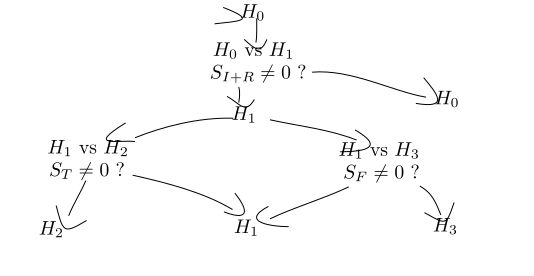
\includegraphics[width=0.7\linewidth]{./img_diagramas/estacionariedad_decidir.pdf}
%\caption{Representaci\'on diagram\'atica de la implementaci\'on en R de la prueba PSR. Se omite 
%filtrado previo mediante el algoritmo STL (ver texto).}
\label{diagrama_psr}
\end{figure}

\begin{figure}
\centering
\begin{lstlisting}[caption={}]
Priestley-Subba Rao stationarity Test for datos
-----------------------------------------------
Samples used              : 3072 
Samples available         : 3069 
Sampling interval         : 1 
SDF estimator             : Multitaper 
  Number of (sine) tapers : 5 
  Centered                : TRUE 
  Recentered              : FALSE 
Number of blocks          : 11 
Block size                : 279 
Number of blocks          : 11 
p-value for T             : 0.4130131 
p-value for I+R           : 0.1787949 
p-value for T+I+R         : 0.1801353 
\end{lstlisting}
\caption{Resultado mostrado tras una ejecuci\'on de la funci\'on \texttt{stationarity}.
El par\'ametro \texttt{n.blocks} define la cantidad grupos disjuntos para los cuales se 
calcular\'a el estimador de la FDE.
Cabe resaltar el antepen\'ultimo rengl\'on (\texttt{p-value for T}), seg\'un el cual se puede
aceptar o rechazar la hip\'otesis de estacionariedad d\'ebil.
La FDE es referida como 'Spectral Density Function' (SDF).}
\label{res_psr}
\end{figure}

\begin{figure}
\centering
\includegraphics[width=0.7\linewidth]{./img_diagramas/psr_simple.pdf}
\caption{Representaci\'on diagram\'atica de la implementaci\'on en R de la prueba PSR. Se omite 
filtrado previo mediante el algoritmo STL (ver texto).}
\label{diagrama_psr}
\end{figure}

%%%%%%%%%%%%%%%%%%%%%%%%%%%%%%%%%%%%%%%%%%%%%%%%%%%%%%%%%%%%%%%%%%%%%%%%%%%%%%%%%%%%%%%%%%%%%%%%%%%
%%%%%%%%%%%%%%%%%%%%%%%%%%%%%%%%%%%%%%%%%%%%%%%%%%%%%%%%%%%%%%%%%%%%%%%%%%%%%%%%%%%%%%%%%%%%%%%%%%%
%%%%%%%%%%%%%%%%%%%%%%%%%%%%%%%%%%%%%%%%%%%%%%%%%%%%%%%%%%%%%%%%%%%%%%%%%%%%%%%%%%%%%%%%%%%%%%%%%%%
%%%%%%%%%%%%%%%%%%%%%%%%%%%%%%%%%%%%%%%%%%%%%%%%%%%%%%%%%%%%%%%%%%%%%%%%%%%%%%%%%%%%%%%%%%%%%%%%%%%
